\documentclass[]{beamerruhuisstijl}

\title{Erik de NaoButler}
\author{Robin Immel, Camil Staps}

\begin{document}
\frame{\titlepage}

\begin{frame}
  \frametitle{Algemene info Nao}
  \begin{itemize}
    \item Aldebaran
    \item 7000 exemplaren verkocht
    \item Meerdere versies aanwezig, elk met een andere toevoeging
    \item Voorloper Pepper  
  \end{itemize}
\end{frame}

\begin{frame}
  \frametitle{Uitleg idee}
  \begin{itemize}
    \item Een robot butler
    \item Dynamisch opstellen herkenningspunten
  \end{itemize}
\end{frame}

\begin{frame}
  \frametitle{Ons algoritme}
  \begin{itemize}
    \item Twee versies
      \begin{itemize}
        \item Van woonkamer naar keuken $\to$ Oplopende nummers volgen
        \item Van keuken naar woonkamer $\to$ Aflopende nummers volgen
      \end{itemize}
    \item Als de Nao een landmark ziet zal hij er naartoe (proberen) te lopen
    \item Wanneer er geen landmark gevolgd wordt, ronddraaien en zoeken naar nieuw punt 
  \end{itemize}

  \begin{center}
    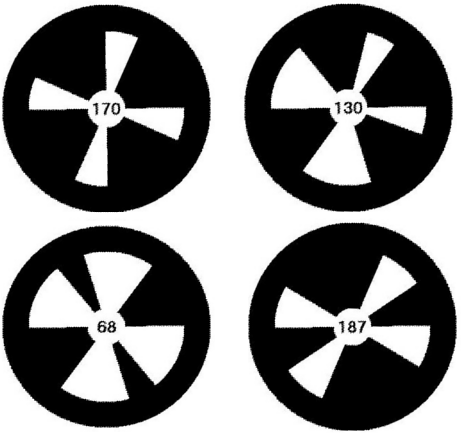
\includegraphics[width=.25\linewidth]{naomark}
  \end{center}
\end{frame}

\begin{frame}
  \frametitle{Unieke eigenschappen}
  \begin{itemize}
    \item Sociale interactie door middel van een interne database
    \item Dynamisch kunnen aanmaken en verplaatsen landmarks
    \item Zelf customizen van rugzak
  \end{itemize}
\end{frame}

\begin{frame}
  \frametitle{Demo}
\end{frame}

\begin{frame}
  \frametitle{Meevallende aspecten}  
  \begin{itemize}
    \item Lopen zit al enigszins in de Nao
    \item Landmarks makkelijk om te zetten tot beacons
      \begin{itemize}
        \item Pre-made rondjes die door Nao herkend worden
        \item Te printen vanaf de cd
        \item Door papieren vorm makkelijk en snel te verplaatsen
      \end{itemize}
  \end{itemize}
\end{frame}

\begin{frame}
  \frametitle{Tegenvallende aspecten}  
  \begin{itemize}
    \item Langzaam opladen
    \item Lopen werkt na een redelijk korte periode minder soepel
    \item Moeilijk verbinden met netwerk, waardoor code uploaden moeilijker is dan verwacht
    \item Sporadisch omvallen zonder enige reden
  \end{itemize}
\end{frame}


\begin{frame}
  \frametitle{Uitdagingen project}  
  \begin{itemize}
    \item Bestuderen en goed gebruik maken van API
    \item In de praktijk leren wat wel en niet mogelijk is
      \begin{itemize}
        \item Door gesloten systeem niet echt een duidelijk framework
        \item Ondergrond leek meerdere keren niet handig voor Nao's voetjes
      \end{itemize}
    \item Zelf veel ontdekken/maken van custom functies door kleine community
  \end{itemize}
\end{frame}

\begin{frame}
  \frametitle{Verdere uitbreidingen}
  \begin{itemize}
    \item Eén keer met landmarks lopen, route onthouden
    \item Obstacle avoidance
    \item Ondersteuning voor meer dan twee doelen
    \item Rugzakje
  \end{itemize}
\end{frame}

\begin{frame}
  \frametitle{Vragen?}
\end{frame}
\end{document}
